% !TeX root = RJwrapper.tex
\title{Reproducible Summary Tables with gtsummary}
\author{by Daniel D. Sjoberg, Karissa Whiting, Michael Curry}

\maketitle

\abstract{
An abstract of less than 150 words.
}

\section{Introduction}

\section{Data Summaries}

To show use of gtsummary functions, we will use a simulated clinical trial data set containing baseline characteristics of 200 patients who received Drug A or Drug B as well as the outcome of tumor response to the treatment.
Each variable in the data frame has been assigned an attribute label (i.e. \texttt{attr(trial\$trt, "label") == "Chemotherapy Treatment"}) with the labelled[add ref] package. 
These labels are displayed in the {gtsummary} tables by default. Using {gtsummary} on a data frame without labels will print variable names in place of variable labels with the option to update the text displayed.

% adding table describing trial dataset
\captionsetup[table]{labelformat=empty,skip=1pt}
\begin{longtable}{llll}
\toprule
colname & label & class & values \\ 
\midrule
\texttt{trt} & Chemotherapy Treatment & character & \texttt{Drug A}, \texttt{Drug B} \\ 
\texttt{age} & Age & numeric & \texttt{6}, \texttt{9}, \texttt{10}, \texttt{17}, ... \\ 
\texttt{marker} & Marker Level (ng/mL) & numeric & \texttt{0.003}, \texttt{0.005}, \texttt{0.013}, \texttt{0.015}, ... \\ 
\texttt{stage} & T Stage & factor & \texttt{T1}, \texttt{T2}, \texttt{T3}, \texttt{T4} \\ 
\texttt{grade} & Grade & factor & \texttt{I}, \texttt{II}, \texttt{III} \\ 
\texttt{response} & Tumor Response & integer & \texttt{0}, \texttt{1} \\ 
\texttt{death} & Patient Died & integer & \texttt{0}, \texttt{1} \\ 
\texttt{ttdeath} & Months to Death/Censor & numeric & \texttt{3.53}, \texttt{5.33}, \texttt{6.32}, \texttt{7.27}, ... \\ 
\bottomrule\caption{\label{tab:caption}Table 1. Example data frame, \texttt{trial}}\\

\end{longtable}



\subsection{\texorpdfstring{\texttt{tbl\_summary()}}{tbl\_summary()}}

The default output from \texttt{tbl\_summary()} is meant to be publication ready.
The \texttt{tbl\_summary()} function can take, at minimum, a data frame as the only input, and returns descriptive statistics for each column in the data frame.
This is often the first table of clinical manuscripts and describes characteristics of the cohort under study.
A simple example is shown below.
Notably, by specifying the \texttt{by=} argument, you can stratify the summary table. 
In the example below, we have split the table by the treatment a patient received. 

% code for basic tbl_summary()
\begin{example}
trial %>%
  select(age, grade, response, trt) %>%
  tbl_summary(by = trt)
\end{example}
\begin{figure}[h!]
  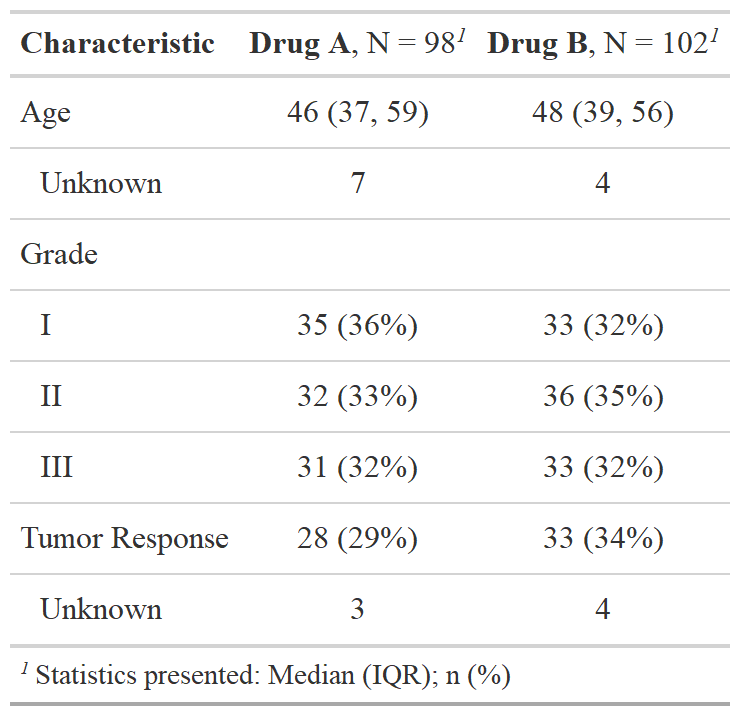
\includegraphics[height=5cm]{summary_basic.png}
  \centering
\end{figure}

The function is highly customizable, and it is initiated with sensible default settings.
Specifically, \texttt{tbl\_summary} detects variable types of input data and calculates descriptive statistics accordingly.
For example, variables coded as \texttt{0/1}, \texttt{TRUE/FALSE}, and \texttt{Yes/No} are presented dichotomously.
Additionally, \texttt{NA} values are recognized as missing and listed as unknown, and if a data set is labelled, the label attributes are automatically utilized. 

Default settings may be customized using the \texttt{tbl\_summary()} function arguments.

% code for tbl_summary() with arguments
\captionsetup[table]{labelformat=empty,skip=1pt}
\begin{longtable}{ll}
\toprule
Argument & Description \\ 
\midrule
\texttt{label=} & specify the variable labels printed in table \\ 
\texttt{type=} & specify the variable type (e.g., continuous, categorical, etc.) \\ 
\texttt{statistic=} & change the summary statistics presented \\ 
\texttt{digits=} & number of digits the summary statistics will be rounded to \\ 
\texttt{missing=} & whether to display a row with the number of missing observations \\ 
\texttt{missing\_text=} & text label for the missing number row \\ 
\texttt{sort=} & change the sorting of categorical levels by frequency \\ 
\texttt{percent=} & print column, row, or cell percentages \\ 
\texttt{include=} & list of variables to include in summary table \\ 
\caption{\label{tab:}\texttt{tbl\_summary()} function arguments}\\
\bottomrule
\end{longtable}



In the example below, continuous variables are cast to \texttt{"continuous2"}, meaning the continuous summary statistics will appear on two or more rows in the table.
The \texttt{"age"} variable's label is updated to \texttt{"Patient Age"}.
Default summary statistics for both continuous and categorical variables are updated using the \texttt{statistic=} argument.
The \texttt{digits=} argument is used to increase the number of decimal places the statistics are rounded, and the missing row is omitted with \texttt{missing = "no"}.

\begin{example}
trial %>%
  select(age, grade, response, trt) %>%
  tbl_summary(
    by = trt,
    type = all_continuous() ~ "continuous2",
    label = age ~ "Patient Age",
    statistic = list(all_continuous() ~ c("{N_nonmiss}", 
                                          "{mean} ({sd})", 
                                          "{median} ({p25}, {p75})", 
                                          "{min}, {max}"),
                     all_categorical() ~ "{n} / {N} ({p}%)"),
    digits = all_categorical() ~ c(0, 0, 1),
    missing = "no"
  )
\end{example}
\begin{figure}[h!]
  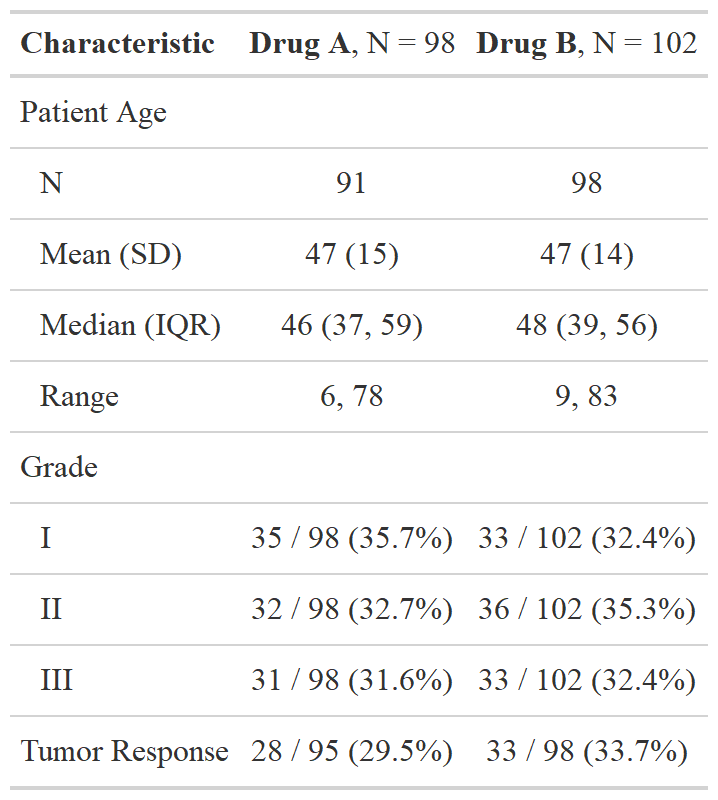
\includegraphics[height=5cm]{summary_plus.png}
  \centering
\end{figure}

\textbf{A note about notation:}
Throughout the gtsummary package, you'll find function arguments that accept a list of formulas (or a single formula) as the input.
In the example above, the label for the age variable was updated using \texttt{label = age $\sim$ "Patient Age"}---equivalently, \texttt{label = list(age $\sim$ "Patient Age")}.
To select groups of variables, utilize the select helpers from the tidyselect[add ref] and gtsummary.
Above, \texttt{all\_continuous()} was utilized to change the summary statistics for all continuous variables. 
Similarly, users may utilize \texttt{all\_categorical()} (from gtsummary), or any of the tidyselect helpers used throughout the tidyverse[add ref] package, such as \texttt{starts\_with()}, \texttt{contains()}, etc.

The gtsummary package has several functions to add information or statistics to \texttt{tbl\_summary()} tables.

% code for tbl_summary() with arguments
\captionsetup[table]{labelformat=empty,skip=1pt}
\begin{longtable}{ll}
\toprule
Function & Description \\ 
\midrule
\texttt{add\_p()} & add \emph{p}-values to the output comparing values across groups \\ 
\texttt{add\_overall()} & add a column with overall summary statistics \\ 
\texttt{add\_n()} & add a column with N (or N missing) for each variable \\ 
\texttt{add\_difference()} & add column for difference between two group, confidence interval, and \emph{p}-value \\ 
\texttt{add\_stat\_label()} & add label for the summary statistics shown in each row \\ 
\texttt{add\_stat()} & generic function to add a column with user-defined values \\ 
\texttt{add\_q()} & add a column of \emph{q}-values to control for multiple comparisons \\ 
\bottomrule\caption{\label{tab:caption}Table 3. \texttt{tbl\_summary()} functions to add information}\\

\end{longtable}



In the example below the number of non-missing observations is reported for each variable, as well as a p-value comparing the values between the treatment.
The \texttt{add\_p(pvalue\_fun=)} argument accept both a proper function as well the formula shortcut notation used through the tidyverse packages.

\begin{example}
trial %>%
  select(age, grade, response, trt) %>%
  tbl_summary(by = trt, missing = "no") %>%
  add_n() %>%
  add_p(test = all_continuous() ~ "t.test",
        pvalue_fun = ~style_pvalue(., digits = 2))

\end{example}
\begin{figure}[h!]
  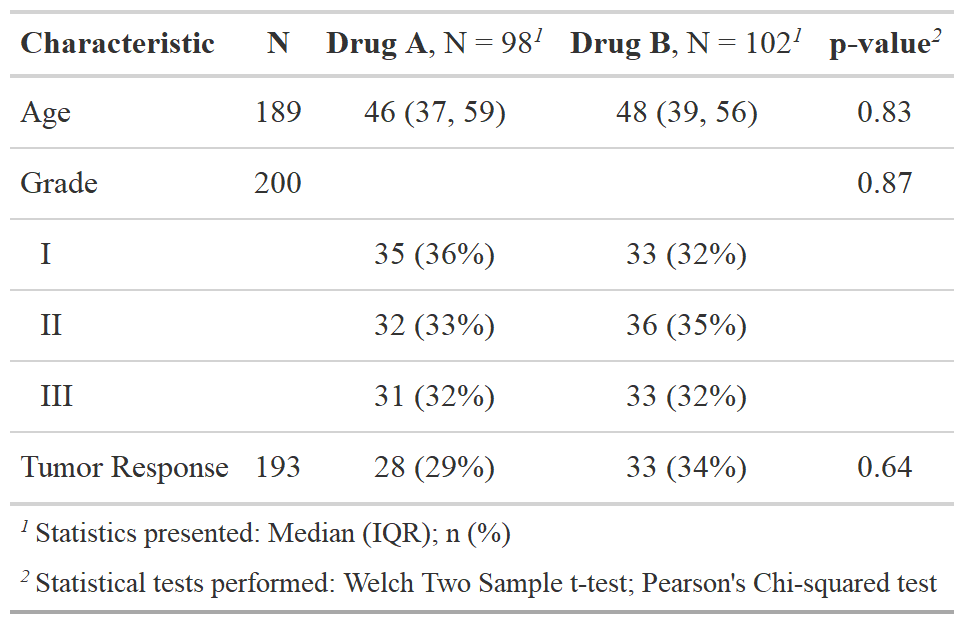
\includegraphics[height=5cm]{summary_plus_plus.png}
  \centering
\end{figure}

\subsection{\texorpdfstring{\texttt{tbl\_svysummary()}}{tbl\_svysummary()}}

The \texttt{tbl\_svysummary()} function is very similar to \texttt{tbl\_summary()} except a survey object is supplied rather than a data frame.

\begin{example}
# create weighted survey object, keep only two counties
data(api, package = "survey")
svy_api <- 
  survey::svydesign(id = ~dnum, weights = ~pw, data = apiclus1, fpc = ~fpc) %>%
  subset(cname %in% c("Alameda", "Los Angeles"))

# summarize data
svy_api %>%
  tbl_svysummary(by = cname, 
                 include = c(growth, target, cname),
                 label = list(growth ~ "Growth",
                              target ~ "Target")) %>%
  add_p()
\end{example}
\begin{figure}[h!]
  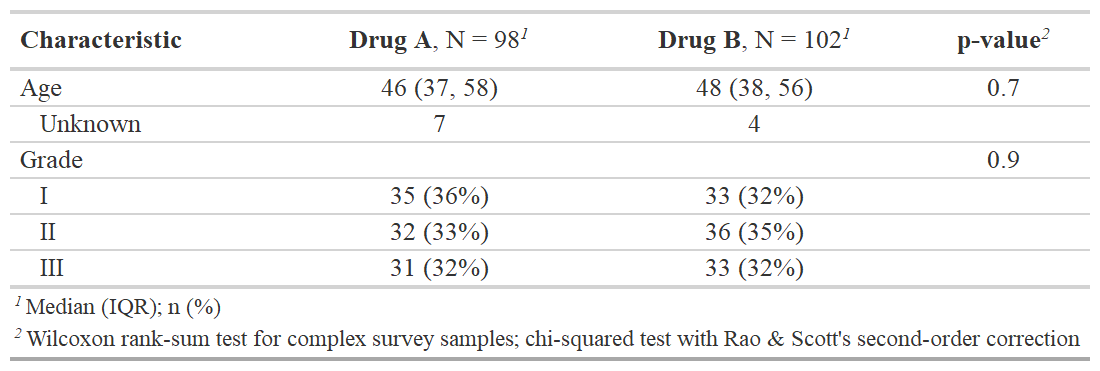
\includegraphics[height=4cm]{svysummary.png}
  \centering
\end{figure}

\subsection{\texorpdfstring{\texttt{tbl\_cross()}}{tbl\_cross()}}

The \texttt{tbl\_cross()} function continues using similar syntax as the previous functions, resulting in a cross tabulation table ready for publication. 

\begin{example}
trial %>%
  tbl_cross(row = stage, col = trt, percent = "cell") %>%
  add_p(source_note = TRUE)
\end{example}
\begin{figure}[h!]
  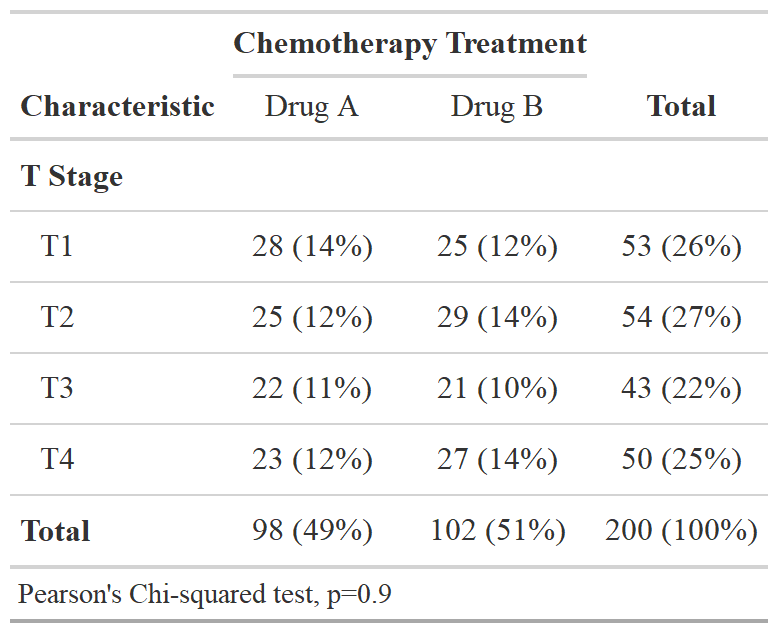
\includegraphics[height=4cm]{cross.png}
  \centering
\end{figure}

\subsection{\texorpdfstring{\texttt{tbl\_survfit()}}{tbl\_survfit()}}

The \texttt{tbl\_survfit()} parses and tabulates n-year survival and survival percentile estimates from \texttt{survival::survfit()}.


\begin{example}
library(survival)

list(survfit(Surv(ttdeath, death) ~ trt, trial),
     survfit(Surv(ttdeath, death) ~ grade, trial)) %>%
  tbl_survfit(times = c(12, 24),
              label_header = "**{time} Month**") %>%
  add_p()
\end{example}

% TODO: I do not understand why this isn't being placed below the code! https://www.overleaf.com/learn/latex/Positioning_of_Figures
\begin{figure}[h!]
  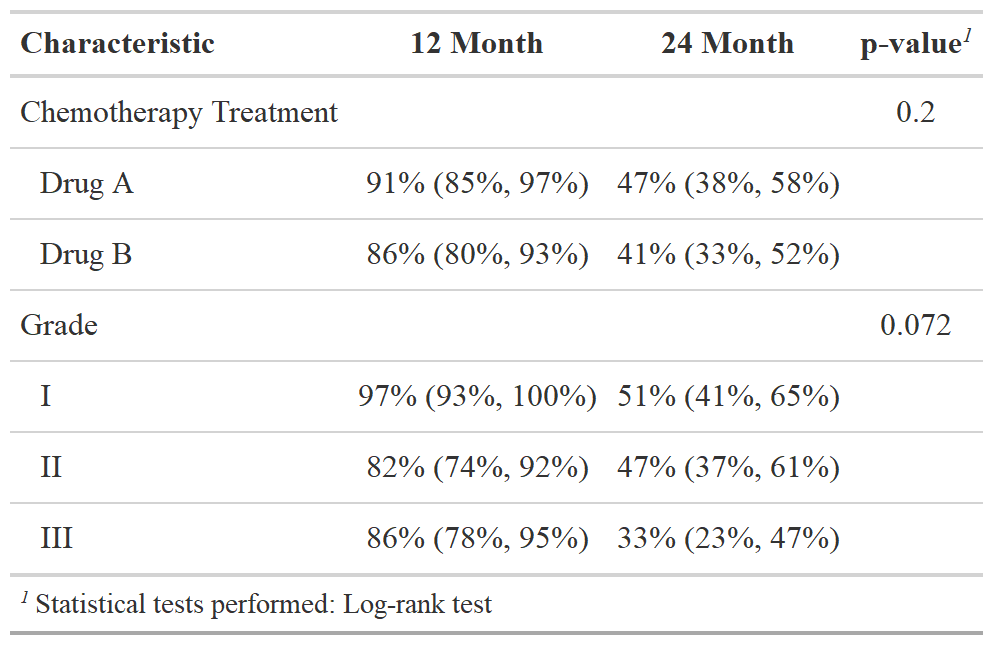
\includegraphics[height=4cm]{survfit.png}
  \centering
\end{figure}

\subsection{Customization}

% adding table describing fns for customization
\captionsetup[table]{labelformat=empty,skip=1pt}
\begin{longtable}{ll}
\caption{\label{tab:} Functions to style and modify gtsummary tables}\\
\toprule
Function & Description \\ 
\midrule
\texttt{modify\_header()} & update column headers \\ 
\texttt{modify\_footnote()} & update column footnote \\ 
\texttt{modify\_spanning\_header()} & update spanning headers \\ 
\texttt{modify\_caption()} & update table caption/title \\ 
\texttt{bold\_labels()} & bold variable labels \\ 
\texttt{bold\_levels()} & bold variable levels \\ 
\texttt{italicize\_labels()} & italicize variable labels \\ 
\texttt{italicize\_levels()} & italicize variable levels \\ 
\texttt{bold\_p()} & bold significant p-values \\ 
\bottomrule
\end{longtable}



\section{Model Summaries}

\subsection{\texorpdfstring{\texttt{tbl\_regression()}}{tbl\_regression()}}

\begin{example}
glm(response ~ age + grade, trial, family = binomial) %>%
  tbl_regression(exponentiate = TRUE) %>%
  add_global_p()
\end{example}

\begin{figure}[h!]
  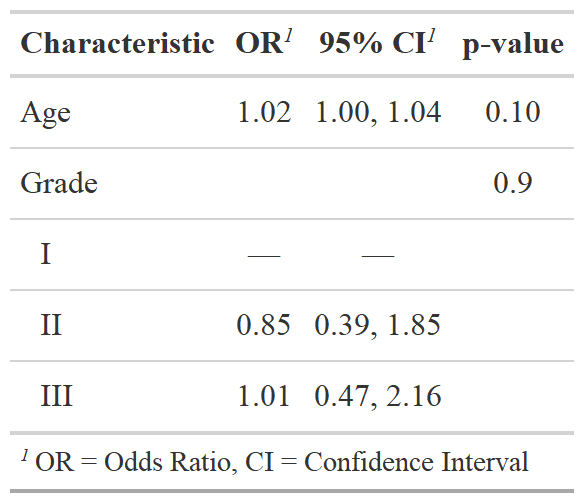
\includegraphics[height=4cm]{regression.png}
  \centering
\end{figure}

\subsection{\texorpdfstring{\texttt{tbl\_uvregression()}}{tbl\_uvregression()}}
\begin{example}
trial %>%
  select(response, age, grade) %>%
  tbl_uvregression(
    y = response, 
    method = glm,
    method.args = list(family = binomial),
    exponentiate = TRUE,
    pvalue_fun = ~style_pvalue(., digits = 2)
  ) %>%
  add_nevent() %>%
  add_global_p()
\end{example}

\begin{figure}[h!]
  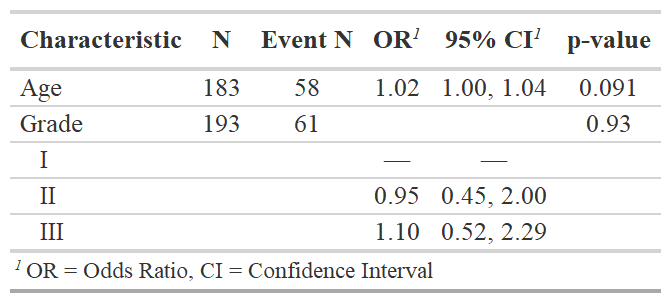
\includegraphics[height=4cm]{uvregression.png}
  \centering
\end{figure}

\hypertarget{in-line-reporting}{%
\section{In-line Reporting}\label{in-line-reporting}}

\hypertarget{merging-and-stacking}{%
\section{Merging and Stacking}\label{merging-and-stacking}}

\hypertarget{themes}{%
\section{Themes}\label{themes}}

\hypertarget{print-engines}{%
\section{Print Engines}\label{print-engines}}

\bibliography{RJreferences}

\address{Daniel D. Sjoberg\\
  Memorial Sloan Kettering Cancer Center\\
  1275 York Ave., New York, New York 10022\\
  USA\\
  ORCID 0000-0003-0862-2018\\
  \email{sjobergd@mskcc.org}}

\address{Karissa Whiting\\
  Memorial Sloan Kettering Cancer Center\\
  1275 York Ave., New York, New York 10022\\
  USA\\
  ORCID 0000-0002-4683-1868\\
  \email{author2@work}}

\address{Michael Curry\\
  Memorial Sloan Kettering Cancer Center\\
  1275 York Ave., New York, New York 10022\\
  USA\\
  ORCID 0000-0002-0261-4044\\
  \email{author3@work}}
